\section{Zielsetzung}
\label{sec:Zielsetzung}

Spurdetektoren wie Szintillatoren werden in der experimentellen Physik dazu verwendet, die Bewegungsbahn und Energie
von Teilchen zu untersuchen. Durch diese Informationen lassen sich Rückschlüsse auf die zugrundeliegenden Zerfälle und
beteiligten Teilchen ziehen. In dieser Versuchsreihe wird eine szintillierende Faser auf bestimmte Eigenschaften
untersucht und schließlich durch die gewonnenen Erkenntnisse eine vorhandene Simulation einer szintillierenden Faser
der Realität angepasst.

\section{Theorie}
\label{sec:Theorie}

Mithilfe von szintillierender Fasern können Impuls und Position elektrisch geladener Teilchen ermittelt werden
und somit beispielsweise die Masse bestimmt werden. Diese Methode wird seit 2019/2020 an dem LHCb-Experiment 
verwendet, um mitunter CP-verletzende Zerfälle zu erforschen. Die TU Dortmund ist an der Entwicklung 
des SciFi (Scinitillating Fiber) Trackers stark involviert. Eine wichtige Eigenschaft des SciFi Trackers ist 
seine Auflösung, welche besser als $\qty{100}{\micro\metre}$\cite{SciFi_Versuch} ist.

\subsection{Anordnung und Aufbau}

Die einzelnen Szintillator Fasern haben einen Durchschnitt von $\qty{250}{\micro\metre}$, welcher sich aus einem
$\qty{220}{\micro\metre}$ dicken Kern aus Polystyrol und zwei Ummantelungen mit einer Dicke von $\qty{7.5}{\micro\metre}$
zusammensetzt. Die Fasern werden zu mehreren Fasermatten zusammengefügt, wobei ein hexagonales Muster
verwendet wird, um möglichst wenig leere Zwischenräume zu erzeugen und die Raumauflösung zu maximieren. Die einzelnen Faser Lagen
werden mit Epoxy-Kleber zusammengehalten. Eine schematische Darstellung dieser Anordnung ist in \autoref{pic:Anordnung_Matte} zu sehen.

\begin{figure}
    \centering
    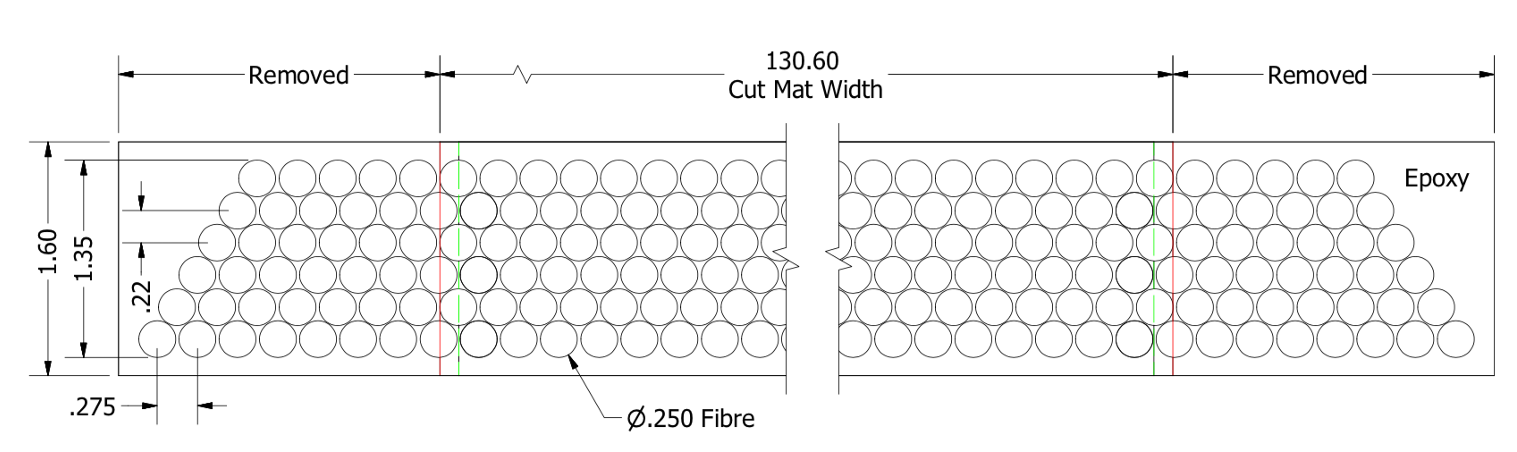
\includegraphics[width = .8\textwidth]{content/pics/Anordnung.png}
    \caption{Schematische Darstellung der Anordnung der einzelnen Fasern innerhalb der Fasermatten \cite{SciFi_Versuch}.}
    \label{pic:Anordnung_Matte}
\end{figure}
Der SciFi Tracker besteht aus den Tracker Stationen T1-T3, welche hintereinander angeordnet sind. Die einzelnen 
Stationen bestehen widerum aus vier Lagen an Fasermatten, welche in einem x-u-v-x Muster angeordnet sind. Die Lagen u und v
sind hierbei um jeweils $\pm 5°$ zu den x-Lagen rotiert. Jede Lage umfasst jeweils 40 nebeneinander angeordnete Matten und zwei übereinander
angeordnete Schichten. An den inneren Enden jeder Matte sind Spiegel angebracht, welche das erzeugte Photonensignal 
reflektieren. An den jeweiligen äußeren Enden befinden sich Silizium Photomultiplier, um das Signal auszuwerten. Die Anordnung
der Fasermatten-Lagen ist in \autoref{pic:Lagen_Anordnung} gezeigt.
\begin{figure}
    \centering
    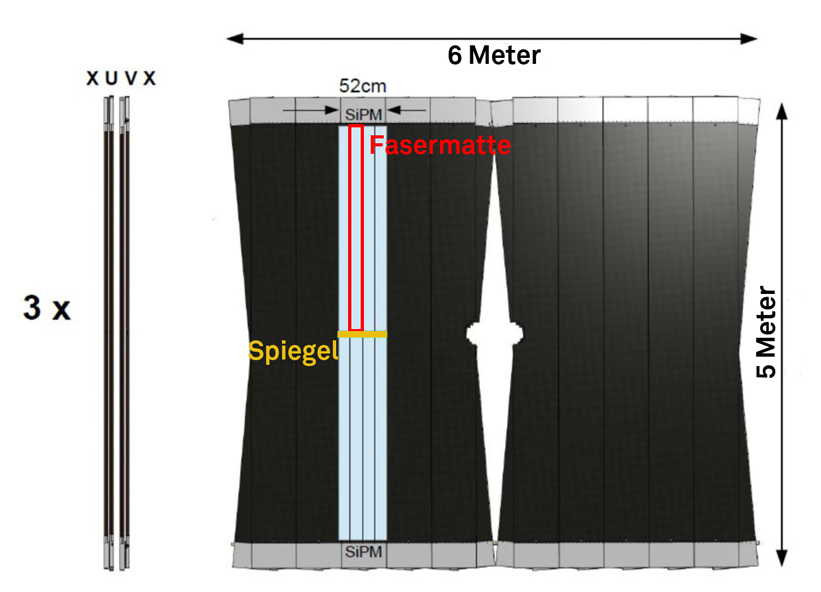
\includegraphics[width = .8\textwidth]{content/pics/Lagen_Anordnung.png}
    \caption{x-u-v-x Struktur der Fasermatten-Lagen (links) und der Aufbau einer Tracking Station (rechts) \cite{SciFi_Versuch}.}
    \label{pic:Lagen_Anordnung}
\end{figure}

\subsection{Funktionsweise}

Die Fasern bestehen in ihrem Kern aus Polystyrol. Polystyrol ist ein organischer Szintillator, welcher bei dem 
Durchflug geladener Teilchen Photonensignale erzeugt. Bei organischen Szintillatoren werden diese Signale durch
molekulare Vorgänge produziert. Hierbei zeigt sich bei längerer Bestrahlung eine Strukturänderung und ein Leistungsabfall des
Detektors, was durch Alterungserscheinungen hervorgerufen wird. Anorganische Szintillatoren zeigen keine solche Erscheinungen,
sind aber aus Kostengründen für ein so großen Detektor wie der LHCb Detektor ungeeignet.\\
Die Funktionsweise organischer Szintillatoren beruht auf der Anregung von Molekülzuständen, welche bei Relaxation
Photonen im UV-Bereich emittieren. Bei Polystyrol werden die Valenzelektronen, auch $\pi$-Elektronen genannt, angeregt.
Diese Elektronen sind in Benzolringen delokalisiert und können sich frei im Polystyrol-Molekül bewegen. Diese Elektronen
werden durch elastische Stöße entweder in einen $S_{10} - S_{13}$ oder $S_{20} - S_{22}$ Zustand angeregt. Die Moden $S_{11} - S_{13}$ und $S_{20} - S_{22}$
gehen hierbei schnell strahlungsfrei wieder in den $S_{10}$ Zustand über. Bei Relaxationen des $S_{10}$ Zustands in den 
Grundzustand $S_{00}$ werden schließlich Photonen im UV-Bereich emittiert.\\
Da lediglich $3 \, \%$ der angeregten Elektronen in den Zustand $S_{00}$ relaxieren und dabei UV-Photonen
emittieren, wird dem Polystyrol der Farbstoff p-Terphenyl hinzugefügt. Durch diesen Farbstoff verkürzt sich die Zerfallsdauer
von $\qty{308}{\nano\second}$ auf wenige Nanosekunden. Hierdurch wird die erwünschte Relaxation nicht mehr durch 
schneller ablaufende strahlungsfreie Zerfälle dominiert. Die Energieniveaus der $\pi$-Elektronen ist schematisch in 
\autoref{pic:Energieniveaus} dargestellt.

\begin{figure}
    \centering
    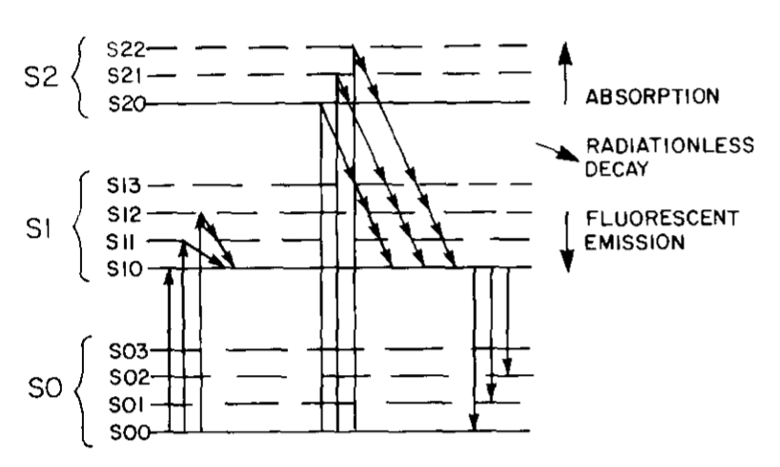
\includegraphics[width = .8\textwidth]{content/pics/Energieniveaus.png}
    \caption{Energieniveaus der $\pi$-Elektronen in Polystyrol \cite{SciFi_Versuch}.}
    \label{pic:Energieniveaus}
\end{figure}
UV-Strahlung besitzt in durchsichtigen Materialien eine zu geringe Reichweite, als dass ausreichend viele Photonen die Photomultiplier
erreichen. Daher wird ein Wellenlängenschieber verwendet, um die Wellenlänge auf einen langwelligeren Bereich
zu projezieren. Hierfür muss das Emissionsspektrum des p-Terphenyl und das Absorptionsspektrum des Wellenlängenschiebers
möglichst übereinstimmen. Durch diesen Prozess wird die durchschnittliche Reichweite der Photonen erhöht, sodass
ein Großteil die Photomultiplier das Ende der Fasern erreicht. Die Emissions- und Absorptionsspektren von Polystyrol,
p-Terphenyl und dem verwendeten Wellenlängenschieber TPB ist in \autoref{pic:Spektren} dargestellt.
\begin{figure}
    \centering
    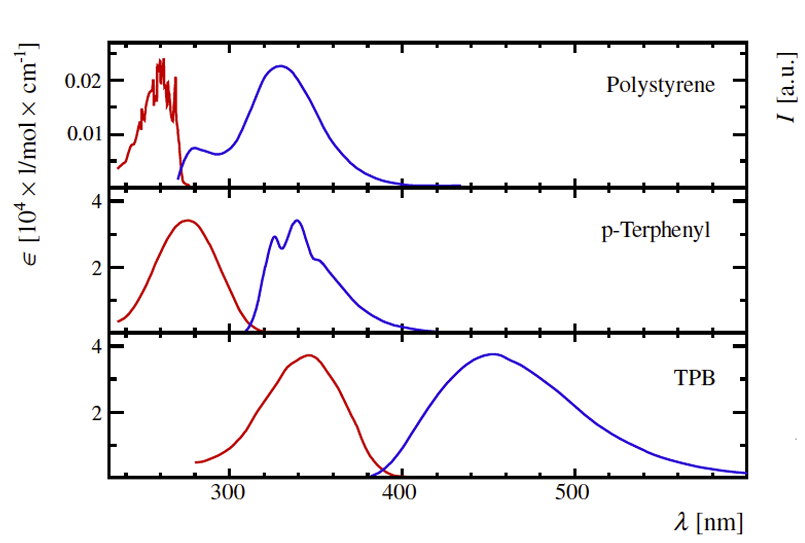
\includegraphics[width = .8\textwidth]{content/pics/Spektren.png}
    \caption{Absorptions- (rot) und Emissionsspektren (blau) von Polystyrol, p-Terphenyl und TPB \cite{SciFi_Versuch}.}
    \label{pic:Spektren}
\end{figure}

\subsection{Signalweiterleitung}

Die Photonen werden innerhalb der Faser mittels Totalreflexionen weitergeleitet. Totalreflexion
tritt hierbei ab einem Grenzwinkel auf, welcher durch das Snelliussche Brechungsgesetz hergeleitet werden kann:
\begin{align}
    \label{eq:Snellius}
    \frac{\sin{\delta_2}}{\sin{\delta_1}} &= \frac{n_1}{n_2} \, , \, \delta_2 = \frac{\pi}{2} \\
    \Rightarrow \sin{\delta_{\text{g}}} &= \frac{n_2}{n_1},
\end{align}
wobei $n_1$ der Brechungsindex des Mediums der einlaufenden Welle ist und $n_2$ der des Mediums der auslaufenden
Welle. $\delta_1$ ist der Winkel der einlaufenden Welle zum Lot auf der Grenzfläche, $\delta_2$ der Winkel der auslaufenden
Welle zum Lot und $\delta_{\text{g}}$ der Grenzwinkel. Die gegebene Situation ist schematisch in \autoref{pic:Snellius} dargestellt.\\
\begin{figure}
    \centering
    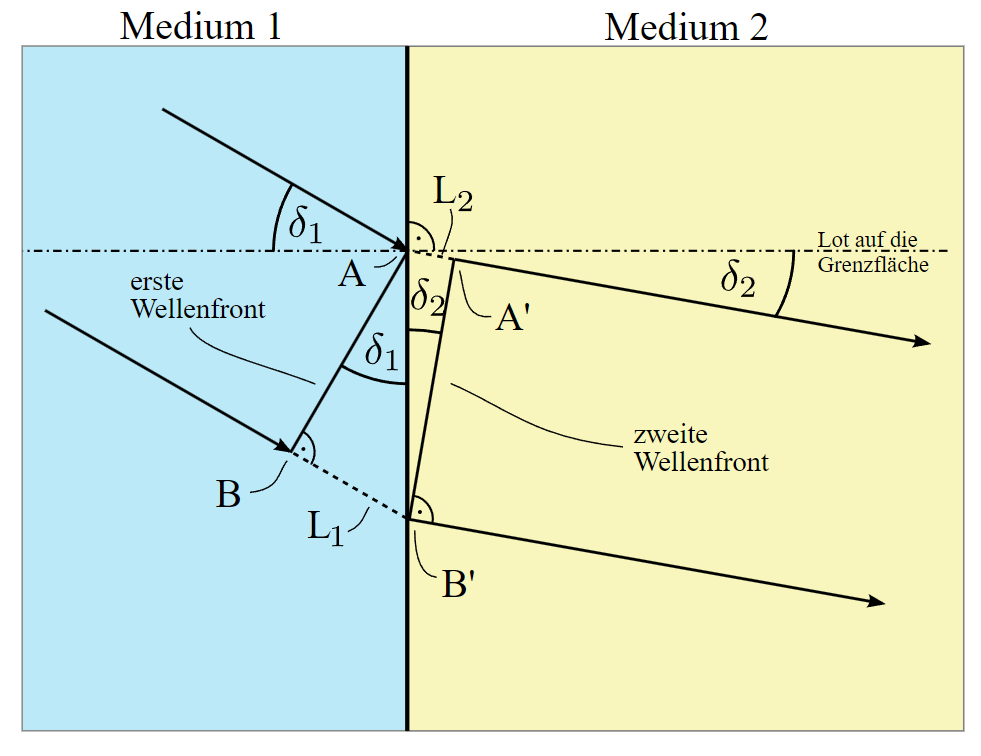
\includegraphics[width = .5\textwidth]{content/pics/Snellius.png}
    \caption{Schematische Darstellung der Reflexion und Brechung von elektromagnetischen Wellen beim Übergang in ein anderes Medium \cite{Snellius}.}
    \label{pic:Snellius}
\end{figure}
Bei der effektiven Betrachtung der Faser werden Reflexionen an der Grenzfläche zwischen äußerer Ummantelung und der Umgebungsluft vernachlässigt, da der
Epoxy-Kleber dort keine Totalreflexionen zulässt. Für die zurückgelegte Strecke der Photonen $L$ und die Anzahl der Reflexionen innerhalb
der Faser $N$ lässt sich
\begin{align}
    \label{eq:rel}
    L &= \frac{x}{\cos{\Theta}}\\
    N &= \frac{x \tan{\Theta}}{2 \sqrt{r^2_{\text{Kern}} - r^2_{\text{min}}}} \label{eq:N}
\end{align}
bestimmen. Hier ist $\Theta$ der Winkel zur Fasermittelachse, $r_{\text{Kern}}$ der Radius des p-Terphenyl Kerns und $r_{\text{min}}$ der kleinste
Abstand der Photonen zur Mittelachse der Faser. $r_{min}$ kann nicht experimentell ermittelt werden. Mithilfe einer Simulation kann allerdings
ein mittlerer Wert ermittelt werden.\\
Je größer der kleinste Abstand des Photons zu der Mittelachse ist, desto eher bewegt sich dieses auf einer Kreisbahn, was zur Konsequenz hat,
dass solche Photonen auch noch über dem ermittelten Grenzwert Totalreflexionen ausführen können. Wenn man solche Bahnen mit $r_{\text{min}} \neq 0$ berücksichtigt,
ergibt sich die Gleichung
\begin{equation}
    \Theta_{\text{refl}} = \arcsin{\left(\sqrt{1 - \frac{r^2_{\text{min}}}{r^2_{\text{Kern}}}} \sin{\Theta}\right)}.
\end{equation}

\subsubsection{Verlusteffekte}

Bei der Propagation von Photonen durch Materie können mehrere Effekte auftreten, die die mittlere Reichweite innerhalb der Faser beeinflussen.
Einer dieser Effekte ist die Rayleigh-Streuung, bei der elektromagnetische Strahlung an einem Teilchen gestreut wird, wenn dessen Wellenlänge
kleiner ist als die Wellenlänge des Photons. Durch diese Ablenkung kann es dadurch kommen, dass Photonen nicht länger den richtigen Winkel zu den
Grenzflächen haben, um Totalreflexionen ausführen zu können. Weiterhin kann es durch Anregung von Molekülschwingungen oder Selbstabsorption
des Wellenlängenschiebers zu einer Abschwächung der Intensität des Signals kommen. Die Abschwächung der Intensität durch diese Mechanismen lässt sich
mit einem Absorptionskoeffizienten $a$ darstellen. Für die Intensität der Photonen gibt es eine exponentielle Abhängigkeit
zum Absorptionskoeffizienten, welche durch
\begin{equation}
    I(x) = I_0 \exp\left(-\frac{x}{\lambda}\right)
\end{equation}
gegeben ist. $\lambda$ ist die Abschwächlänge und wird durch das Inverse des Absorptionskoeffizienten berechnet. Bei den verwendeten Fasern
liegt diese bei etwa $\qty{3.5}{\metre}$ \cite{SciFi_Versuch}. Diese Verlustmechanismen treten sowohl bei der Propagation durch das Kernmaterial,
als auch bei der Reflexionen an der Ummantelung auf. Da diese zwei Fälle unterschiedliche Winkelabhängigkeiten besitzen, können sie
getrennt betrachtet werden. Die Verluste im Kernmaterial sind gegeben durch
\begin{equation}
    A_{\text{Kern}}(x, \Theta) = \exp{\left(- \frac{L(x,\Theta)}{\lambda}\right)}
\end{equation}
und die Reflexionsverluste an der Grenzfläche zur Ummantelung durch
\begin{equation}
    A_{\text{refl}}(x, \Theta) = \exp{\left(N(x,\Theta) \ln{(1-\epsilon)}\right)} \approx \exp{\left( -N(x,\Theta) \epsilon \right)}.
\end{equation}
$\epsilon$ ist der Reflexionskoeffizient, welcher die Wahrscheinlichkeit angibt, dass ein Photon bei der Reflexion an der Ummantelung absorbiert wird.
Somit ergibt sich durch Muliplikation der beiden Effekte und Verwendung der ausdrücke für $L$ und $N$ (\autoref{eq:rel} und \ref{eq:N}) die totale Intensität nach
\begin{equation}
    I(x,\Theta) = I_0  \exp{\left( - \frac{L(x,\Theta)}{\lambda}-N(x,\Theta) \epsilon \right)} = I_0  \exp{\left(-x \left( \frac{1}{\lambda\cos{\Theta}}+\frac{ \tan{\Theta}\epsilon}{2 \sqrt{r^2_{Kern} - r^2_{min}}} \right) \right)}.
\end{equation}
Es kann schließlich eine effektive Abschwächung definiert werden als
\begin{equation}
    \label{eq:absorption}
    a_{\text{eff}} = \frac{a_0}{\cos{\Theta}} + \frac{\epsilon \tan{\Theta}}{2 \sqrt{r^2_{\text{Kern}} - r^2_{\text{min}}}}.
\end{equation}
Bei einem Winkel von $\Theta$ verschwinden, wie zu erwarten, jegliche Reflexionsverluste. Daher können die Verluste innerhalb des Kerns
isoliert und ohne Einfluss der Reflexionsverluste untersucht werden.

\subsection{Silizium Photomultiplier}

Zur Detektion der erzeugten und weitergeleiteten Photonen werden Silizium Photomultiplier (SiPMs) verwendet. Diese befinden sich an den äußeren 
Enden der Fasermatten. Diese Photomultiplier sind im Geiger-Modus betriebene Avalanche-Photodioden. Die Photomultiplier bestehen aus mehreren 
Pixeln, welche jeweils einen Raum von $\qty{57.7}{} \times \qty{62.5}{\micro\metre}$ abdecken. Jeder Pixel besteht aus einem pn-Übergang, welcher
beim Eintreffen eines Photons eine messbare Spannung erzeugt. Der zugrundeliegende Prozess entsteht durch einen p- und n-dotierten Halbleiter.
An diesem wird eine Spannung angelegt und somit eine Raumladungszone erzeugt in der keine freien Elektronen vorliegen. Regt ein Photon ein Elektron
der Raumladungszone an, so entsteht ein Elektron-Loch-Paar. Das Elektron wird durch die angelegte Spannung zu der Kathode beschleunigt
und regt auf seinem Weg weitere Elektronen an. Hierdurch können Ladungslawinen von circa $10^6$ Elektronen entstehen, welche detektiert werden.\\
Der Halbleiter benötigt etwa $\qty{25}{\nano\second}$, um sich von einer Ladungslawine zu relaxieren und erneut Photonen detektieren zu können.
Die Pixelgröße muss optimiert sein, da bei zu großen Pixeln zu viele Photonen ein Signal aussenden und es bei zu kleinen Pixeln dazu kommen kann,
dass benachbarte Pixel ebenfalls eine Ladungslawine auslösen.\\
Jeweils mehrere Pixel sind entlang der Bewegungsrichtung der Photonen in Kanäle aufgeteilt. Für die Auswertung werden jeweils alle gefeuerten Pixel
pro Kanal aufsummiert und als Signalstärke interpretiert. Aus den Signalstärken wird die mittlere Position berechnet und somit eine Bahn rekonstruiert.
Dieser Prozess ist in \autoref{pic:Pixel} simuliert. \\

\begin{figure}
    \centering
    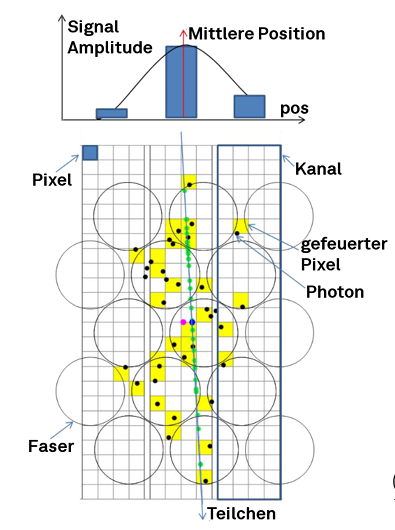
\includegraphics[width = .4\textwidth]{content/pics/Pixel_kanal.png}
    \caption{Simulation der Photonendetektion durch einzelne Pixel der Photomultiplier. \cite{SciFi_Versuch}}
    \label{pic:Pixel}
\end{figure}

Mithilfe der Photodetektionseffizienz (PDE) lässt sich eine Aussage über die Qualität eines Detektors bilden. Sie gibt das Verhältnis zwischen 
detektierten und tatsächlich auftreffenden Photonen an. Die Wellenlängenabhängigkeit der PDE ist in \autoref{pic:PDE} dargestellt.\\

\begin{figure}
    \centering
    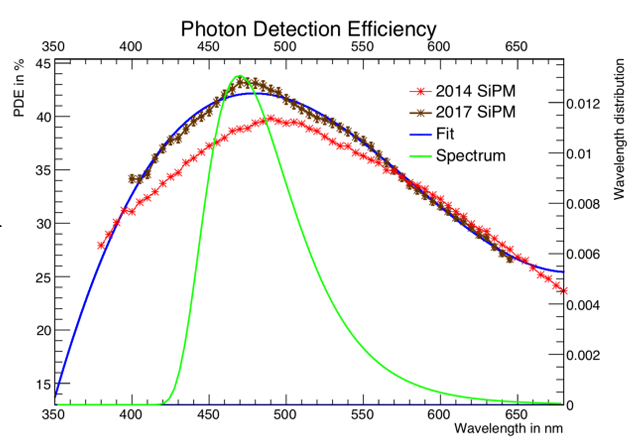
\includegraphics[width = .8\textwidth]{content/pics/PDE.png}
    \caption{Photonendetektoreffizienz in Abhängigkeit der Wellenlänge \cite{SciFi_Versuch}.}
    \label{pic:PDE}
\end{figure}

Wichtig ist zudem die Dunkelstromrate, welche die ausgelösten Signale ohne tatsächlich eintreffende Photonen beschreibt. Diese entsteht durch
thermische Photonen und ist dadurch stark temperaturabhängig. Die Silizium Photomultiplier werden daher auf $-40 \, ° \mathrm{C}$ abgekühlt.\\
Um eine wellenlängenabhängige Messung zu erhalten, müssen winkelabhängige Messungen mit einem Spektrometer durchgeführt werden, welches Wellenlängen auflösen kann.

\subsection{Simulation der Fasern}

Mithilfe von Monte-Carlo Simulationen können simulierte Photonen durch einen simulierten Detektor geschickt werden und dadurch Daten erhalten
werden, ohne tatsächliche, echte Messungen durchführen zu müssen. Die hier verwendeten Simulationsdaten sind Simulationen einzelner szintillierender
Fasern und wurden in GEANT4 erstellt. Es wurden einzelne Photonen simuliert und die verschiedenen theoretischen Verlustmechanismen berücksichtigt,
um möglichst realitätsnahe Ergebnisse zu erhalten. Die verwendete Simulationsdaten bestehen aus 50 Fasern mit je 24 Anregungspunkten. Diese
Anregungspunkte sind jeweils $\qty{100}{\milli\metre}$ voneinander entfernt. Die erzeugten simulierten Messdaten können schließlich mit echten 
verglichen werden, um die Simulation von unphysikalischen Ereignissen zu bereinigen und zu optimieren. Aus der Simulation können verschiedene Objektattribute
als Variablen zu Auswertung verwendet werden.